\chapter{Design}
\label{chap:design}
In diesem Kapitel werden die Anforderungen präzisiert und ein Design für die Umsetzung erarbeitet.
Dazu sind mehrere Aspekte relevant: zum einen die technische Umsetzung der Filterung und Generierung von Dumps (Architektur und unterstützte Filterkriterien), sowie das User-Interface und welche externen Dienste genutzt werden können (z.B. für die Archivierung der erzeugten Dumps).
Diese bedingen sich gegenseitig: es ist wenig sinnvoll, wenn die Architektur sehr komplexe Filterkriterien unterstützt, dass User-Interface das aber gar nicht abbilden kann (oder umgekehrt).

\section{Architektur}
Für die Architektur der Anwendung stellt sich zuerst die Frage, wie die Arbeit zwischen Server und Client verteilt werden soll.
Auf der einen Seite steht die Variante, einen schlauen Client zu entwickeln, welcher direkt mit der Wikidata API und dem SPARQL-Endpunkt spricht bzw. den Dump als Stream verarbeitet.
Der Client kann dann von jedem Nutzer lokal auf seinem eigenen System ausgeführt werden.
Der Vorteil dieser Variante ist eindeutig: der Server müsste in diesem Fall keine eigenen Dumps erzeugen, sondern maximal Metadaten zu generierten Dumps speichern.
Allerdings bringt diese Variante auch mehrere Probleme: erstens muss der Client vom Nutzer selbst ausgeführt werden, was problematisch wird wenn die Erzeugung der Dumps einen längeren Zeitraum in Anspruch nimmt, da dann das System des Nutzers die gesamte Zeit online sein muss.
Zweitens müsste für die Archivierung der Nutzer die Dumps selbst hochladen.
Die Generierung auf einem Server hat diese Nachteile nicht.
Der Nutzer muss während der Generierung nicht online sein, sondern kann den Dump einfach herunterladen sobald dieser fertig ist.
Außerdem kann die Archivierung vom Server übernommen werden.
Die umgesetzte Anwendung implementiert die Logik zur Generierung der Dumps daher auf dem Server.

Für die Generierung der Dumps auf dem Server sind drei Varianten denkbar:
\begin{enumerate}[label=\alph*) ]
  \item Der Server verwaltet einen eigenen Index
  \item Der Server nutzt den Wikidata SPARQL Endpunkt und die Wikidata API
  \item Der Server verarbeitet die existierend JSON- oder RDF-Exporte von Wikidata auf Anfrage sequentiell
\end{enumerate}
Variante a) könnte zum Beispiel so aussehen, dass die Daten vorher in kleine Blöcke zerlegt werden, von denen dann nur die gewünschten kombiniert werden.
Insgesamt hat diese Variante den Vorteil, dass die Erzeugung der Dumps sehr schnell geht, denn es müssen nur die geforderten Blöcke gelesen werden.
Allerdings ist die Variante relativ komplex zu implementieren, da der Index mit den aktuellen Daten von Wikidata synchron gehalten werden muss.
Dazu ist entweder eine periodische Neuerstellung notwendig oder der Index muss inkrementell aktualisiert werden, was die Komplexität weiter erhöht.
Die Notwendigkeit der inkrementellen Aktualisierung und des gezielten Zugriff auf Teile der Daten hindert außerdem die Kompression.
Diese Variante hat damit einen hohen Speicherplatzbedarf.

Variante b) basiert auf der Beobachtung, dass die Indexierung der Daten genau das ist, was auch RDF-Datenbanken machen.
Es gibt schon eine existierende RDF-Datenbank für die Daten von Wikidata, die über den Wikidata Query Service abgefragt werden kann.
Diese wird auch ständig aktuell gehalten, was das Problem der Aktualität löst.
Die Generierung der Dumps in dieser Variante würde aus den Filterkriterien einen SPARQL-Query generieren und diesen dann an den SPARQL-Endpunkt von Wikidata senden.
Wie auch Variante a) ist diese Möglichkeit sehr schnell, der Wikidata SPARQL Endpunkt besitzt ein Timeout von 60 Sekunden.
Genau das ist aber auch ein Problem dieser Variante: das Timeout von 60 Sekunden erlaubt es nicht, sehr große Mengen von Daten über den Query Service anzufragen. Zum Beispiel terminiert diese Abfrage, welche alle Instanzen der Klasse \verb|Q13442814| (wissenschaftlicher Artikel) abfragt, nicht innerhalb des Timeouts (das Ergebnis wären 21986127 Entities):
\begin{lstlisting}[language=SPARQL, caption=SPARQL-Query nach wissenschaftlichen Artikeln]
SELECT ?item {
  ?item wdt:P31 wd:Q13442814
} 
\end{lstlisting}
Zu den Items müssten dann auch noch die Statements und Referenzen abgerufen werden, die in diesem Query noch gar nicht betrachtet werden.

Die Variante c) hat dieses Problem nicht.
Dafür ist hier die Generierung von Dumps deutlich langsamer, da für die Generierung ein vollständiger Wikidata-Export verarbeitet werden muss.
Der Vorteil dieser Lösung ist, dass sie im Vergleich zu Variante a) einfacher in der Umsetzung ist, da keine Synchronisation oder komplexe Indexstrukturen notwendig sind.
Zudem ist kein zusätzlich Speicherbedarf für einen Index erforderlich, der Wikidata-Export kann direkt als Datenstrom verarbeitet werden.
Im Gegensatz zu Variante b) müssen die Filterkriterien nicht als SPARQL formulierbar sein, sondern können in der Programmiersprache implementiert werden, die für die Verarbeitung der Exports genutzt wird.
Dafür sind komplexe, graph-basierte Filter, die das Betrachten von mehr als einer Entität auf einmal erfordern, nicht so einfach umsetzbar.

Die Auswahl der Architektur ist auch davon abhängig, welche Kriterien zur Filterung unterstützt werden sollen.
Ein paar Beispiele von Kriterien, nach denen andere Arbeiten die Exporte von Wissensgraphen wie Wikidata gefiltert haben, sind:
\begin{enumerate}[label=\arabic*)]
  \item nur "`truthy"' Statements mit Entities als Objekt, Labels/Beschreibungen nur in Englisch und Spanisch\cite{usage-grafa}
  \item nur "`truthy"' simple Statements, wobei sowohl Subjekt als auch Objekt ein Wikidata-Item sind\cite{usage-wembedder}
  \item alle Items mit einem Statement für die Property \verb|P727| (Europeana ID, ID in der europäischen virtuellen Bibliothek „Europeana“ für Kulturobjekte)\cite{usage-europeana}
  \item alle Items mit einem Statement für mindestens eine von 50 Properties\cite{usage-narratives} 
  \item nur der englische Teil\cite{usage-web-tables} 
  \item nur Statements für Properties, wobei die Properties Instanzen einer bestimmten Klasse sein müssen, ohne deprecrated, no-value und unknown-value Statements\cite{usage-implicational-knowledge} (allerdings wurde der Dump hier nicht als RDF, sondern in der JSON-Form verarbeitet)
  \item nur Entities von gestorbenen Personen, die an mindestens drei Statements für mindestens 5000 mal vorkommende Properties beteiligt sind\cite{usage-learning-structured-embeddings}
  \item kleinere Datensätze, erzeugt durch zufälliges Auswählen von Statements\cite{usage-sparql-benchmark}
  \item alle Items, die Instanzen (\verb|P31|) der Klassen \verb|Q5| (Mensch) sind und mindestens 6 Fakten (Statements) haben\cite{usage-one-sentence} oder nur die einfachen Statements dieser Personen für die Properties \verb|P27| (Land der Staatsangehörigkeit) und \verb|P106| (Tätigkeit)\cite{usage-person-networks}
  \item zufällige Auswahl von Entities (Sampling), mit englischer Beschreibung und mindestens 5 Statements\cite{usage-generate-entity-type-desc}, optional auch mit Downsampling von Instanzen bestimmter Klassen (um die Verteilung der Klassen im Ergebnis auszugleichen)\cite{usage-synthesize-entity-desc}
  \item alle Statements, welche Referenzen haben, und die Sitelinks der Subjekte dieser Statements\cite{wd-wk-common-references}
\end{enumerate}
Alle diese Filter sind für jede Entität lokal auswertbar, es müssen keine benachbarten Entitäten angeschaut werden.
Nur die Entscheidung, für welche Properties die Statements exportiert werden sollen, ist teilweise komplizierter.
Bei einer sequentiellen Verarbeitung von Dumps ist die Zugehörigkeit einer Property zu einer Klasse erst bekannt, sobald die Entität für diese Property verarbeitet wurde.
Da die Anzahl der Properties jedoch gering genug ist (< 10000), können solche komplexe Filter vor Beginn der Verarbeitung mithilfe des Wikidata Query Service in eine Liste von Properties aufgelöst werden.
Die Variante c) kann damit die Filter dieser Art abdecken.
Auch Sampling (zufällige Auswahl eines Subsets der Daten) kann in dem sequentiellen Ansatz einfach implementiert werden.

Insgesamt bietet der sequentielle Ansatz die meiste Flexibilität und ist einfach in der Implementierung.
Variante a) ist komplizierter und weniger flexibel, da ein Index nur bestimmte Filter effizient unterstützt.
Variante b) funktioniert nur für kleinere Dumps, weil bei größeren Dumps das Problem des Timeouts auftritt.
Die Einfachheit der Variante c) erlaubt es, schnell neue Arten von Filtern zu implementieren.
In dieser Arbeit wurde sich deshalb für diese Variante entschieden, auch da zu erwarten ist, dass das System am Anfang noch keine Nutzung in so großem Ausmaß haben wird, um die Komplexität und den zusätzlichen Speicherbedarf eines Index zu rechtfertigen.

\section{Interface}
Das Interface hat die Aufgabe, die Erstellung und Spezifikation von Dumps möglichst einfach zu gestalten und bereits existierende Dumps zu finden und anzuzeigen.
Um das Interface für die Spezifikation der Filter zu entwerfen muss zunächst die Struktur der Filter, welche unterstützt werden sollen, genauer festgelegt werden.

Die Anwendungsfälle für das Filtern von Wikidata sind verschieden.
Ein typisches Szenario ist die Extraktion von Daten einer bestimmten Thematik, z.B. nur Daten von Personen oder Städten.
In diesem Fall geschieht die Filterung auf Entitätenebene, mit eventuell zusätzlichen Einschränkung der zu exportierende Statements und Sprachen.
Ein anderes Szenario orientiert sich mehr an der Struktur der Statements.
Beispiele hierfür sind die Analyse von Statements mit mindestens einer Referenz, die Extraktion aller Statements für eine bestimmte Property oder alle Statements mit deprecrated Rank.
Das dritte Szenario verwendet Filterung, um die Daten für Benchmarks auf eine kleinere Menge zu reduzieren.
In diesem Fall sind statistische Filter interessant, um zum Beispiel nur jedes zehnte Statement oder nur jede zehnte Entität zu exportieren.

\begin{figure}
  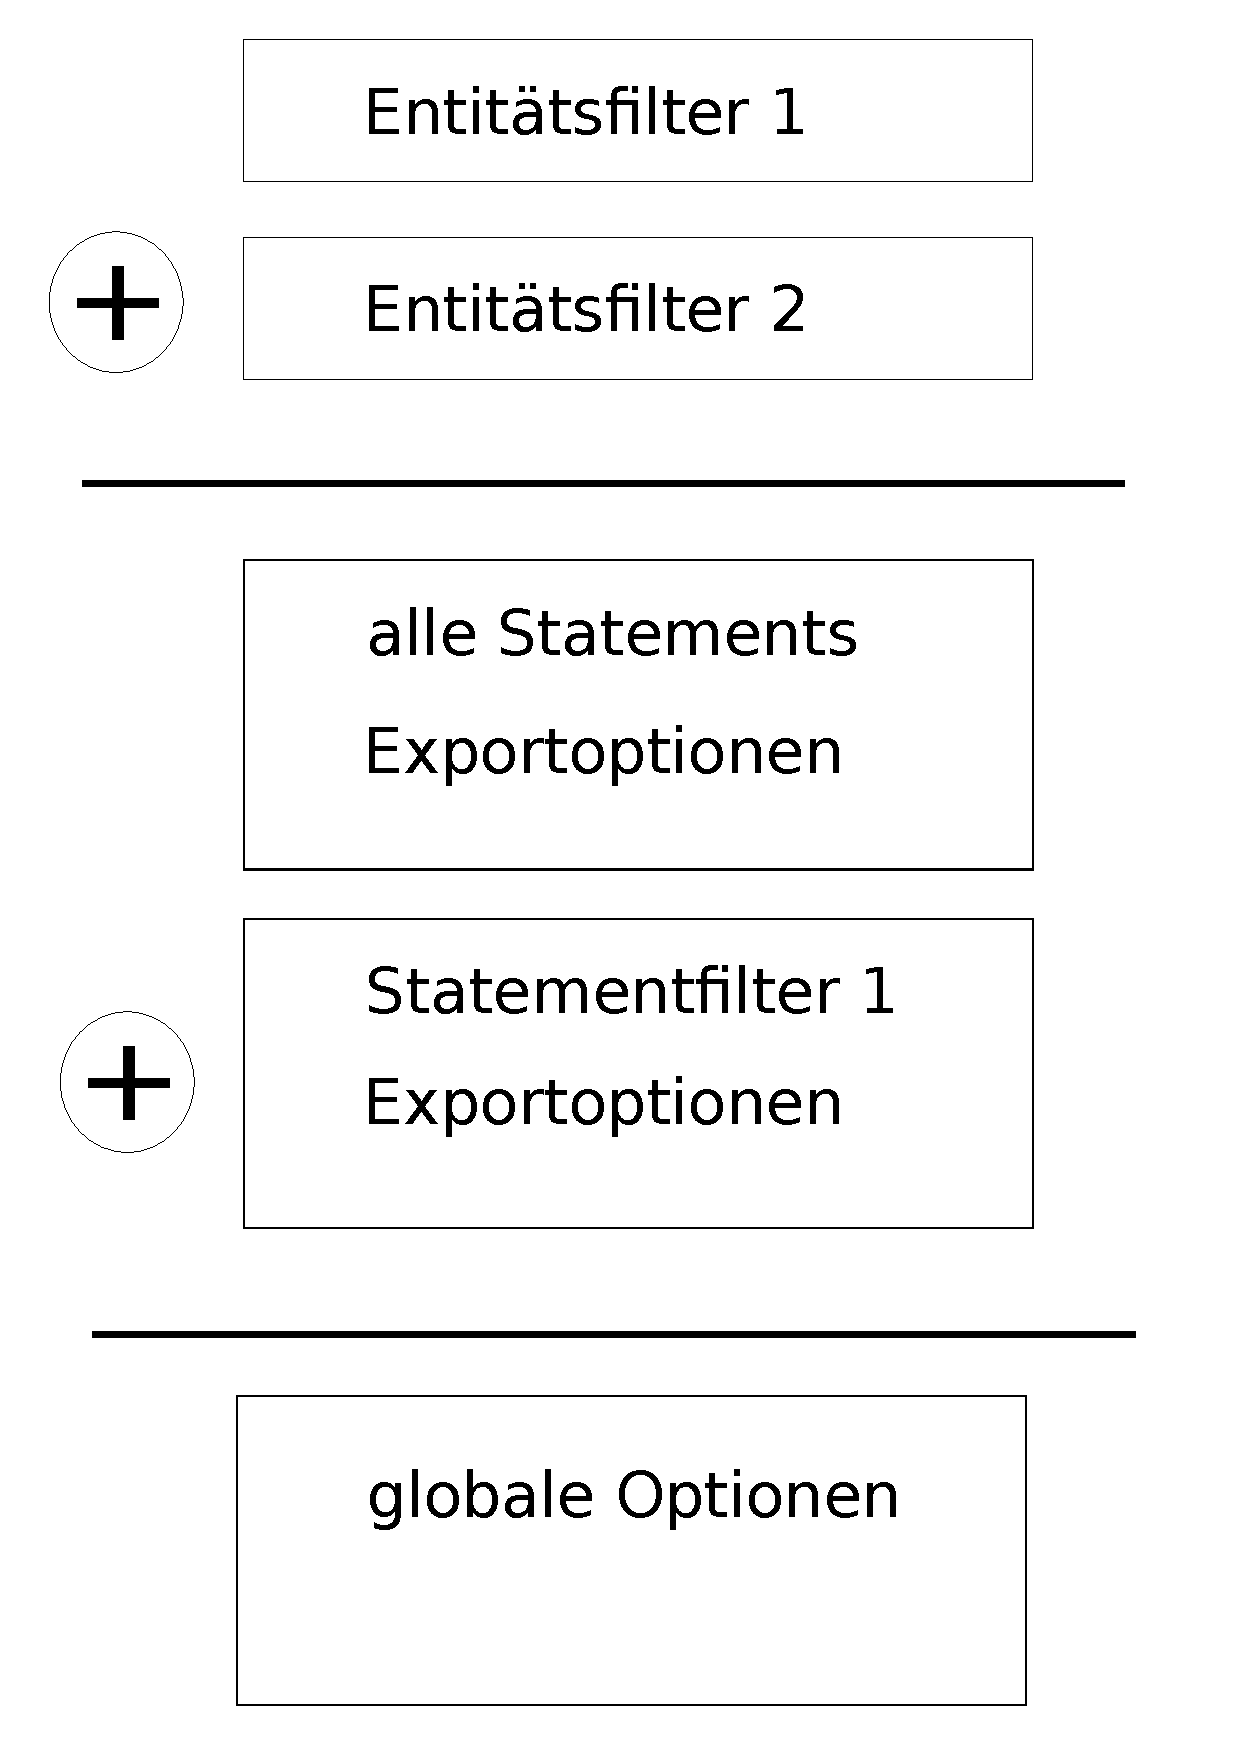
\includegraphics[width=\textwidth]{pics/ui-layout}
  \caption{Struktur des Interfaces zum Erstellen von Dumps}
  \label{fig:ui-layout}
\end{figure}

In Wikidata sind Statements immer ein Teil von Entities.
Folglich kann der Filterprozess konzeptionell in zwei Schritte zerlegt werden: zuerst werden die Entities ausgewählt, danach für diese Entities die zu exportierenden Statements.
Zusätzlich gibt es noch weitere globale Optionen, die sich nicht auf einzelne Statements beziehen, wie bspw. welche Sprachen exportiert werden sollen oder ob sitelinks von Entities exportiert werden sollen.
Diese Struktur des Interfaces ist in \cref{fig:ui-layout} dargestellt.

Für die Auswahl der Entitäten sind viele verschiedene Arten von Bedingungen denkbar.
Deswegen erlaubt das Interface die Kombination mehrerer Entitätsfilter von unterschiedlicher Art.
Für die erste Version der Software ist zunächst eine Filterart geplant, die Auswahlkriterien auf Basis von vorhandenen Statements unterstützt. 
Mit diesem Filter kann gefordert werden, dass Statements für bestimmte Prädikate bzw. bestimmte Prädikat/Objekt-Paare für eine Entität existieren.
Dieser Filter kann als Liste von Bedingungen im Interface dargestellt werden.
Weitere Filter sind denkbar, wie zum Beispiel alle Entitäten die Ergebnis einer SPARQL-Abfrage sind.
Prinzipiell könnte man Filter beliebig mit UND bzw. ODER kombinieren.
Mit dieser Freiheit würde das Interface allerdings sehr komplex.
Um das Interface einfach zu halten, werden Entitätsfilter deshalb immer mit ODER kombiniert, eine Entität wird demnach exportiert wenn mindestens einer der Filter zutrifft.
Es ist auch möglich, keinen Filter anzugeben.
In diesem Fall werden alle Entitäten exportiert (entsprechend den weiteren Regeln).

Für die Statements können Exportoptionen festgelegt werden.
Dafür gibt zum einen Standardoptionen, die für alle Statements der selektierten Entitäten angewendet werden.
Zusätzlich können für bestimmte Prädikate spezielle Exportoptionen festgelegt werden.
Damit können beispielsweise Qualifier nur bei bestimmten Prädikaten exportiert werden.
Die Optionen für den Export von Statements orientieren sich an der Struktur von Wikidata-Statements.
Für jede Komponente eines Statements (simple Statement, full Statement, Qualifier und Referenzen) kann einzeln festgelegt werden, ob diese generiert werden soll oder nicht.
Eine weitere Kategorie von Optionen betrifft den Export von Werten.
Dafür sind Schalter für den Export von einfachen Werten, komplexen Werten, normalisiert oder nicht normalisiert möglich.
Da das Backend das aber noch nicht unterstützt sind diese Optionen im Interface noch nicht vorhanden.
Insgesamt ist dieser Teil aber einfach erweiterbar, da die Optionen alle binär und somit einfach umsetzbar sind.

Die globalen Optionen sind auch größtenteils binär.
Hier kann eingestellt werden, ob Labels, Beschreibungen, Aliase bzw. sitelinks für selektierte Entitäten exportiert werden sollen.
Zudem findet sich hier die Option für die zu exportierenden Sprachen.
Man kann entweder keine Filterung der Sprachen vornehmen (alle Sprachen exportieren) oder eine Liste von Sprachen angeben.

An allen Stellen wo dies sinnvoll ist, bietet das Interface automatische Vervollständigung an.
Das trifft auf alle Eingabefelder für Entitäten zu, wobei Entitäten hier über ihr Label vervollständigt werden.
Außerdem wird eine Vervollständigung bei der Angabe von Sprachen angeboten, wobei eine feste Liste der möglichen Sprachen verwendet wird.

\section{Integration in existierende Infrastruktur}
Um die Anwendung zu betreiben, werden Ressourcen in Form von Rechenzeit für die Generierung der Dumps und Speicherplatz für die Archivierung benötigt.
Dazu lohnt es sich, bereits vorhandene Infrastruktur zu nutzen, um Aufwand und Kosten zu sparen.

Die Anwendung sollte auf Wikimedia-Servern betrieben werden, um die Verfügbarkeit auch in Zukunft unabhängig zu gewährleisten.
Für das Verarbeiten der Dumps und Betreiben des Web-Interfaces bietet sich hier die Wikimedia Toolforge\footnote{\url{https://tools.wmflabs.org/}} an.
Die Toolforge hat eine Grid-Engine, die zum Ausführung von längeren Jobs wie das Verarbeiten der Dumps geeignet ist, eine MySQL-Datenbank und einen Dienst zum Betreiben von Web-Services.
Die Alternative zur Toolforge wäre ein Wikimedia Cloud VPS Projekt\footnote{\url{https://wikitech.wikimedia.org/wiki/Portal:Cloud_VPS}}.
Es wird jedoch empfohlen, Cloud VPS nur zu verwenden, falls die Toolforge nicht ausreichend ist.
Deswegen wird für die Anwendung die Toolforge verwendet, da die Dienste in diesem Fall ausreichend sind.

Für die Archivierung der Dumps ist eine Integration mit Zenodo\footnote{\url{https://zenodo.org/}} vorgesehen.
Zenodo ist ein Datenarchivierungsdienst speziell für wissenschaftliche Zwecke und besitzt auch die Möglichkeit, einen Digital Object Identifier (DOI) zu registrieren, womit die Referenzierung von generierten Datensätzen leicht möglich ist.
Damit wird die Anforderung an Langzeitarchivierung erfüllt. 

Die Integration mit Zenodo funktioniert so, dass abgeschlossene Dumps als Datensatz zu Zenodo hochgeladen werden.
Dabei stellt sich die Frage, welcher Account für den Upload verwendet wird.
Zenodo bietet auch einen OAuth-Schnittstelle an, sodass es möglich wäre, die Dumps direkt zu einem Account des Nutzers hochzuladen.
Das erfordert es allerdings, dass Nutzer bereits einen Zenodo-Account besitzen.
Da die Implementierung von OAuth zudem zusätzliche Komplexität verursacht, verwendet die erste Version der Anwendung einen eigenen Account, der speziell dafür erstellt wurde.
Damit ist es mit einem Klick möglich, einen Dump zu Zenodo hochzuladen und den Dump dann über die DOI zu referenzieren, ohne das die Nutzer selbst einen Account bei Zenodo benötigen.